%2. 31.05-05.06
%* Machine Learning (Features, Labels), Classification, Clustering,
%K-Cross-Validation
%* Verhalten von I/O Systemen (Caches, Wie läuft I/O Kommunikation ab)

\newpage

\section{Grundlagen}
%\todo{Was kommt im Kapitel kurz die (Unter-)Gliederung darstellen}
% machine learning
% decision trees
% caches
% siox activities
\textit{Einige in dieser Arbeit verwendete Begriffe und Techniken sind etwas speziell.
Sie werden deshalb in diesen Abschnitt näher betrachtet.
Als erstes wird das maschinelles Lernen allgemein vorgestellt und dann die Funktionsweise der Entscheidungsbäumen erläutert. 
Es wird die Cachehierarchie und deren Einfluss auf die E/A-Leistung erklärt.
Schließlich werden die Struktur SIOX-Aktivtitäten im Detail betrachtet und dann auf die Erzeugung von Aktivitätsequenzen eingegangen.
}

%Dieser Abschnitt stellt einige Begriffe aus dem Machine-Learning-Bereich vor. 
%Die Definitionen sind an das Buch von Peter Flach \cite{Flach:2012:MLA:2490546} angelehnt.

%%\todo{Worum geht es hier überhaupt?}
%Hier in Prosa erklären, nachher bei Begriffen darauf bezug nehmen.
%Supervised learning, wir wollen etwas über die Eigenschaften einer Menge von Datensätzen lernen um später 
%Eigenschaften eines unvollständigen Datensatzes vorherzusagen.


%Evtl. könnte man hier 
%``Cluster-, Klassifikations- und Regressionsanalyse'' motivieren.
%Aber allgemein langt es vermutlich auch.
\subsection{Maschinelles Lernen}

Beim maschinellen Lernen geht es darum richtigen Datensatz zu finden, um ein richtiges Modell zu bauen, das ein Problem möglichst genaue löst.

% Datensatz
Die Lernalgorithmen setzen in der Regeln eine geeignete Repräsentation der Welt voraus.
Die betrachteten Objekte werden deshalb meistens als eine Reihe von Werten repräsentiert, den s.g. Features.
Einfachheitshalber können sie auch als Messungen von bestimmen Objekteigenschaften gesehen werden, wie z.B. Länge, Anzahl, Geschwindigkeit.
Der Erfolg hängt stark von der Wahl der richtigen Features ab.

% Modell
Die Modelle sind die zentralen Konzepte im Bereich des maschinellen Lernen.
Sie werden trainiert, um bestimmte Aufgaben zu lösen.
Es existiert bereits eine beträchtliche Anzahl von Modellen.
Der Grund für die Vielfalt sind die zahlreichen Problemstellungen, wie z. B. Kategorisierung, Regression, Gruppierung, Assoziationanalyse.
Bei den Modellen handelt es sich im Grunde genommen um die Abbildungen von den Features auf die Ausgabe.

% Aufgabenstellung
Die Aufgabe ist die abstrakte Beschreibung des Problems. 
Sehr oft vorkommende Aufgabenstellung ist beispielsweise die Kategorisierung von Objekten in zwei oder mehrere Kategorien.
Viele Aufgaben können auf die Abbildung von Datenpunkten auf Werte reduziert werden.
Man kann die Algorithmen in drei Klassen unterteilen: unüberwachtes Lernen, überwachtes Lernen und bestärkendes Lernen.
Beim überwachten Lernen stehen dem Algorithmus die Daten und die korrekte Ausgabe zur Verfügung.
Beim unüberwachten Lernen stehen nur die Daten zur Verfügung und der Algorithmus muss die korrekte Ausgabe selber daraus schliessen.
Beim bestärkendem Lernen interagiert der Algorithmus mit der Umgebung und lernt von dem Reaktionen auf seine Handlungen.
Dieser Typ wird allerings in dieser Arbeit nicht verwendet und wurde nur vollständigkeitshalber erwähnt.

\begin{figure}[ht]
	\centering
	\begin{tikzpicture}
	[
		remember picture,
		>=latex reversed,
		-<,
		entity/.style={draw, fill=black!10, rounded corners, minimum height=1cm},
		learnentity/.style={draw, blue, fill=yellow!10, rounded corners, minimum height=1cm},
		gframe/.style={draw, rounded corners, dashed}
	]
	
	\node
		[entity]
		(features)
		{Features};
	\node
		[learnentity, minimum height=0.8cm, right=3.5cm of features]
		(model)
		{Modell};
	\node
		[learnentity, below=of model]
		(alg)
		{Algorithmus};
	
		\begin{pgfonlayer}{background}
			\node
			[entity, minimum width=3cm]
			(model2)
			at (model.center)
			{} ;
		\end{pgfonlayer}

		\coordinate
			[left=3.5cm of features]
			(pstart);
		\coordinate
			[right=3.5cm of model]
			(end);
		\coordinate
			[left=2.3cm of alg]
			(tstart);

		\path 
		(pstart) edge node[above] {Domainobjekte} (features)
			(features) edge node[above] (data) {Daten} (model2)
			(alg) edge (model)
			(model2) edge node[above] (output)  {Ausgabe} (end)
			(tstart) edge[blue] node[above] (dataset) {\color{blue}Datensatz}  (alg);

			\begin{pgfonlayer}{background}
				\node[gframe, loosely dashed, fit=(data) (model) (model2) (output), label=above:{Aufgabe}] {};
				\node[blue, gframe, fit=(dataset) (model) (alg), label=below:{\color{blue}Lernen} ] {};
			\end{pgfonlayer}
\end{tikzpicture}

	\caption{Modell}
	\label{fig:bas:overview}
\end{figure}

Der Zusammenhang zwischen den Aufgaben, Modellen und Lernalgorithmen ist in der \figref{fig:bas:overview} dargestellt. 

In der Trainingsphase trainiert ein Lernalgorithmus das Modell, wobei er ein Datensatz benutzt.
Während der Anwendung werden die Features aus den Objekten extrahiert und an das Modell übergeben.
Das Modell berechnet dann den Ausgabewert.

\subsubsection{Begriffe}

Die wichtigsten Begriffe aus den einleitenden Worten über das maschinelles Lernen werden in den folgenden Definitionen mit mathematischen Elementen erweitert.
Einige Begriffe haben gegenseitige Abhängigkeiten und werden in den Definitionen benutzt bevor sie überhaupt definiert sind.

\begin{term}[Feature und Featuredomain]
	Ein Feature $f_i$ beschreibt eine Eigenschaft des untersuchten Objektes, z.B. kann es das Alter einer Person, die Hausnummer oder die Datenmenge sein. 
	Eine Featuredomain $\mathscr{F}$ legt alle Werte fest, die ein Feature annehmen kann. 
%\todo{Instanz ist der Gegenstand dachte ich, aber das passt dann nicht zu Instanzraum? Ich versuch das mal:}
Mathematisch gesehen handelt es sich um eine Abbildung von dem Instanzraum auf die Featuredomain $f_i : \mathscr{X} \rightarrow \mathscr{F}_i$. 
Mehrere Features bilden ein Featurevektor $x$. 
\end{term}

\begin{term}[Instanzraum]
Der Instanzraum ist ein Kreuzprodukt aus den Featuredomains $\mathscr{X} = \mathscr{F}_1 \times \dots \times \mathscr{F}_d$, wobei die Anzahl der Features $d$ die Dimension des Instanzraumes festlegt.
\end{term}

\begin{term}[Label und Labeldomain]
	Die Featurevektoren können mit einem Label $\mathscr{l}$ behaftet sein. 
	Die Bedeutung des Labels hängt von der Aufgabenstellung ab.
	Die Labeldomain $\mathscr{L}$ legt die gültigen Werte fest, die das Label annehmen kann.
	Es gilt der Zusammenhang $l : \mathscr{X} \rightarrow \mathscr{L}$.
\end{term}


%\begin{term}[Instanz]
%Eine Instanz $S = (F, L)$ ist ein Tupel aus einem Featurevektor und einem Label. 
%Mehrere Instanzen können zu einem Datensatz $\mathcal{S}$ zusammengefasst werden.
%\end{term}

\begin{term}[Modell und Ausgabedomain]
	Ein Modell ist eine Abbildung vom Instanzraum auf die Ausgabedomain $M:\mathscr{X} \rightarrow \mathscr{Y}$.
	Die Ausgabedomain und die Labeldomain sind nicht zwangsläufig gleich.
	Je nach Modelltyp und Lernerfolg können sie von einander abweichen.
\end{term}

\begin{term}[Datensatz]
	Ein Datensatz ist eine echte Untermenge des Instanzraumes $\mathscr{D} \subseteq \mathscr{X}$. 
	Datensätze können aus belabelten oder auch nicht belabelten Features bestehen.
	Sie werden einerseits für das Modelltraining und andererseit zur Validierung des Modell eingesetzt.
	%\todo{Definition... Trainingsdaten, Validierungsdaten?}
\end{term}


\begin{term}[Kreuzvalidierung]
Die Kreuzvalidierung ist eine Auswertungsmethode der Machine-Learning-Algorithmen. 
Die Datensätze werden in $k$ gleiche große Mengen aufgeteilt. 
%\todo{Das ist nicht präzise genug.}
Eine Menge wird für das Training benutzt und $k-1$ Mengen zum Vorhersagen der Werte. 
Die Differenz zwischen den echten und vorhergesagten Werten werden zu einem Durchschnittsfehler zusammengefasst. 
Dieser Schritt wird für die restlichen Mengen durchgeführt und von den $k$ berechneten Durchschnittsfehlern wird ein Durchschnitt berechnet. 
Dieser Wert beschreibt schließlich wie gut der Algorithmus das Problem lösen kann.
\end{term}

\subsubsection{Cluster-, Klassifikations- und Regressionsanalyse}
%\todo{Das würde ich grundsätzlich vorher erklären worum geht es eigentlich?}
Die Clusteranalyse ist eine Prozedur, die eine Menge von Featurevektoren in Gruppen bzw. in die s.g. Cluster eingeteilt. Dabei beinhalten die gleichen Cluster möglichst gleiche Featurevektoren und unterschiedliche Cluster möglichst unterschiedliche. Ein Wissen über die Cluster ist nicht erforderlich.

Die Regressionsanalyse stellt die eine mathematische Beziehung zwischen mehreren unabhängigen Variablen $f$ und einer abhängiger Variable $y$, oder kurz $y = regr(f_1, f_2, \dots, f_n) + e$, wobei $regr$ eine Funktion des Modell ist und $e$ der Fehler.
Die Regressionsanalyse kann eingesetzt werden, um fehlende Werte zu bisher nicht analysieren Variablen vorhersagen.

Die Klassifikationsanalyse ist ein mathematisch-statische Verfahren indem eine untersuchte Einheit, die aus mehreren unabhängigen Variablen $f$ besteht, nach bestimmten Kriterien einer bestimmter Gruppe $y$ zugeordnet wird, oder kurz $y = class(f_1, f_2, \dots, f_n)$, wobei $class$ eine Entscheidungsfunktion des Modell ist. Im Gegensatz zur Regressionsanalyse und Clusteranalyse müssen hier die Klassen bekannt sein und unbekannte Klassen können nicht vorhergesagt werden.


\subsubsection{Entscheidungsbäume}
Einige Algorithmen aus der Entscheidungsbaum-Familie beherrschen sowohl die Klassifizierungs- als auch Regressionsanalyse. 
Sie nutzen zwar unterschiedliche Techniken, um ein Entscheidungsbaum zu erstellen, aber die Entscheidungsbäume funktionieren alle nach demselben Prinzip: 

Als Entscheidungsbäume bestehen aus drei Knotentypen: einer Wurzel, den internen Knoten und den Blättern. 
Jeder interner Knoten hat stets eine oder mehrere Verzweigungen, die als Brücke zu anderen Knoten dienen. 
Jeder interner Knoten ist einem Entscheidungsmerkmal und jeder seiner Zweige ist ein Wertebereich zugeordnet. 
Liegt der Wert des Merkmals im Bereich eines Zweiges, so geht man über ihn zu dem verbundenen Knoten über. 
Die Blätter sind Terminierungsknoten. 
Sie beinhalten die Entscheidungswerte. 

Der Entscheidungsprozess startet immer an der Wurzel, benötigt eine Instanz als Eingabe und liefert stets einen Entscheidungswert als Ausgabe. 
An der Wurzel wird der in aus der Instanz der Wert des Entscheidungsmerkmals entnommen und mit den Wertebereichen des Zweige verglichen. 
Liegt der Wert innerhalb des Wertebereichs eines Zweiges, so geht man über ihn zum nächsten Knoten über. 
Dieser Vorgang wiederholt sich rekursiv bis eine Blatt erreicht wird. Der Wert des Blattes wird zurückgegeben. 

Binärbäume (\figref{fig:bas:decision_tree}) sind besonderere Typen in der Entscheidungsbaumfamilie.
Die interne Knoten in einem Binärbaum besitzen stets zwei Verzweigungen.
Einfachheitshalber, reicht es hier ein Schwellenwert $t$ zu definieren, um zu entscheiden welchen Zweig man folgt.
Wenn $f_i < t$ gilt, dann geht man zum linken Knoten, andernfalls zum rechten.

Die Funktionsweise der Bäume ist relativ einfach und für den Menschen leicht verständlich. 
Man kann nachvollziehen wie bestimmte Entscheidungen zustande kommen und daraus Wissen ableiten. 
Das ist einer der Hauptvorteile der Entscheidungsbäume. 
Ein Beispiel soll es illustrieren.

\begin{figure}[ht]
	\centering
	\begin{tikzpicture}
	[
		remember picture,
		>=latex reversed,
		-<,
		level/.style={sibling distance = 5cm/#1, level distance = 1.5cm}
	]
	
	\node[root](root){I1}
	child{node[internal]{I2} 
		child{node[leaf]{B1}}
		child{node[internal]{I3}
			child{node[leaf]{B2}}
			child{node[leaf]{B3}}
		}
	}
	child{node[internal]{I4}
		child{node[leaf]{B4}}
		child{node[leaf]{B5}}
	};

\end{tikzpicture}

	\caption{Schematische Darstellung eines binären Entscheidungsbaumes.}
	\label{fig:bas:decision_tree}
\end{figure}

\begin{exmp} Ein Beispiel soll die Funktionsweise der Entscheidungsbäume illustrieren.

	\begin{enumerate}
		\item Gegeben sei ein Entscheidungsbaum $M$ (\figref{fig:bas:decision_tree_example}). 
		\item Aufgabe: Berechne $M(x_1)$, mit dem Featurevektor $x_1 = (4, 5, 2)$.
		\item Lösung:
			\begin{enumerate}
				\item An der Wurzel betrachten wir wegen $a = 3$ das dritte Feature $f_3 = 2$.
					Mit dem Schwellenwert $t = 4$ ist die Ungleichung auf dem linken Zweig $f_3 < 4$ erfüllt.
					Wir gehen den Zweig entlang zu den linken Knoten.
				\item Angekommen auf dem linken Knoten, betrachten wir wegen $a = 2$ das zweite Feature $f_2 = 5$. 
					Der Schwellenwert ist hier $t = 2$
					Es gilt die Ungleichung auf dem rechten Zweig $f_2 > 2$, die zum rechnten Knoten führt.
					Wir gehen den Zweig entlang zu den rechten Knoten.
				\item Ein Blatt wurde erreicht.
					Der Entscheidungsbaum gibt den Wert $y = B$.	
				\item Es gilt $M((4, 5, 2)) = B$.
			\end{enumerate}
	\end{enumerate}

	Der Entscheidungsbaum im Beispiel kann die Featurevektoren in drei Kategorien einordnen.
	Für die Kategorisierung allerdings sind nur zwei Features relevant: $f_2$ und $f_3$.
	Das Feature $f_1$ kommt in dem Baum nicht vor und hat keine Auswirkung auf die Ausgabe.
	Wenn das passiert, dass ist das ein deutlicher Hinweis darauf, dass die Features möglicherweise nicht optimal gewählt sind.

\begin{figure}[ht]
	\centering
	\begin{tikzpicture}
	[
		remember picture,
		>=latex reversed,
		-<,
		level/.style={sibling distance = 6cm/#1, level distance = 2cm}
	]
	
	\node[root](root){Wurzel \nodepart{two} $a=3$\\$t=4$}
	child{node[internal]{Int. \nodepart{two} $a=2$\\$t=2$}  
	child{node[leaf]{Blatt \nodepart{two} $y = A$} 
			edge from parent node[left]{$f_2<2$}}
			child{node[leaf]{Blatt \nodepart{two} $y = B$}
			edge from parent node[right]{$f_2 \geq 2$}}
		edge from parent node[left]{$f_3 < 4$}
	}
	child{node[leaf]{Blatt \nodepart{two} $y = C$}
		edge from parent node[right]{$f_3 \geq 4$}};

	\end{tikzpicture}

	\caption{Beispiel.}
	\label{fig:bas:decision_tree_example}
\end{figure}

In diesem einfachen Beispiel kann die Funktionsweise auch graphisch dargestellt werden. 
In der \figref{fig:bas:task} werden die Features $f_2$ und $f_3$ in einem Koordinatensystem aufgespannt.
Die Rechtecke zeigen wie die Kategorien zugeornet werden.

\begin{figure}[ht]
	\centering
	\begin{tikzpicture}[domain=0:11,smooth]
  \begin{axis}[
      width=6cm,height=6cm,
      axis lines=middle,
      domain=0:11,
      smooth,
      no markers,
      %grid,
      xmin=0,xmax=9,
      tick style=black,
      xtick={0, 2,...,8},
      xlabel=$f_2$,
      xlabel style={below, anchor=north east,inner xsep=-10pt},
      restrict y to domain=0:11,
      ymin=0,ymax=9,
			ytick={0, 2,...,8},ylabel=$f_3$,
      ylabel style={above,anchor=north east,inner ysep=-10pt},
      samples=100
    ]

		\begin{pgfonlayer}{background}
			\addplot[const plot mark mid, dashed] coordinates {(0, 4) (9, 4)};
			\addplot[const plot mark mid, draw=none, fill=blue!30] coordinates {(2, 0) (2, 4) (0, 4) (0, 0)} \closedcycle;
			\addplot[const plot mark mid, draw=none, fill=yellow!30] coordinates {(2, 0) (2, 4) (8, 4) (8, 0)} \closedcycle;
			\addplot[const plot mark mid, draw=none, fill=red!30] coordinates {(0, 4) (8, 4) (8, 8) (0, 8)} \closedcycle;
			\addplot[const plot mark mid] coordinates {(0, 4) (8, 4)};
			\addplot[const plot mark mid] coordinates {(2, 4) (2, 0)};
		\end{pgfonlayer}

		\node[fill=white] at (axis cs:1, 2) {$A$};
		\node[fill=white] at (axis cs:5, 2) {$B$};
		\node[fill=white] at (axis cs:4, 6) {$C$};
  \end{axis}

\end{tikzpicture} 

	\caption{Aufgabenstellung.}
	\label{fig:bas:task}
\end{figure}


Aus dem Entscheidungsbaum kann man direkt die Regeln entnehmen.
In diesem einfachen Fall sind es drei folgende Regeln:

\begin{align}
  f_3 < 4 \vee f_2 < 2 &= A\\
	f_3 < 4 \vee f_2 \geq 2 &= B\\
	f_3 \geq 4 &= C
\end{align}
\end{exmp}

\subsection{E/A-Leistung}
Um die E/A-Leistung besser zu verstehen und Missinterpretationen zu vermeiden muss man die grundlegende Funktionsweise der Hardware und Software verstehen und bei der Analyse berücksichtigen. 

\subsubsection{Leistungskennzahlen}
Wegen den unterschiedlichen Einsatzzwecken lässt sich die Leistung der E/A-Systeme nicht durch eine einzige Kennzahl bemessen. 
Stattdessen ist die Leistungskennzahl abhängig vom Systemtypen und muss für jedes System individuell bestimmt werden. 
Die gängigsten Leistungskennzahlen sind:

\begin{term}[Datendurchsatz] % \cite{daver10bu1}]
	Der Datendurchsatz $D$ ist die übertragene Datenmenge pro Zeiteinheit.
	%D = IOPS * IOSize
\end{term}

\begin{term}[Latenz]
	Ist die Zeit zwischen der Adressierung eines Speicherbereiches und der Bereitstellung der Daten.
\end{term}

\begin{term}[Auslastung]
	Die Auslastung $U$ eines Systems ist der Quotient aus der tatsächlicher Nutzungszeit (inkl. Overhead) und der Gesamtzeit. 
\end{term}


\subsubsection{Wahlfrei E/A-Operationen}
Die Massenspeicher können nur eine bestimmte Anzahl der E/A-Operationen pro Sekunde $IOPS$ durchführen. 
% Diese Zahl ist konstant und gibt den Maximalwert an. DAS IST FALSCH, ist nicht konstant.
Bei den Festplatten wird sie z. B. durch die Suchzeit $t_{seek}$ und die Verzögerungszeit $t_{d}$ bestimmt. $t_{seek}$ die der Lesekopf im Schnitt benötigt, um die richtige Spur auf der Scheibe zu finden und $t_d$ ist die Zeit dei im Schnitt vergeht, bis der Lesekopf über die Daten fliegt. IOPS wäre in diesen Fall $IOPS = \frac{1}{t_d + t_{seek}}$.

Da bei jeder E/A-Operation die Datenmenge $d_{size}$ sequentiell durchgeführt wird, lässt sich daraus $IOPS$ und $d_{size}$ der Durchsatz bestimmen.

\begin{equation}
	D = IOPS * d_{size}
\end{equation}



\subsubsection{Einflussfaktoren}
Die E/A-Leistung wird von verschiedenen Faktoren und Parametern beeinflusst, z.B. Blockgröße des Dateisystem, parallele Zugriffe auf das Speicher-Subsystem, Betriebssystem und Anwendungen, Massenspeichercontroller, Speichermediumgeschwindigkeit und -technologie.

% Datenbloecke
%Die Daten werden immer blockweise von Massenspeichermedium gelesen. 
%Die Blockgröße ist abhängig von Systemkonfiguration, der Anwendung oder Betriebssystem. 
%Bei einem eingerichteten System ist die Blockgröße vorgegeben und kann der Benutzer in den meisten Fällen nicht bestimmt werden. 


%\todo{Zuerst die Hardware erklären, dann wird klarer wozu Caches}



\subsubsection{Caches}
% Definition
Caches sind schnelle Zwischenspeicher zur Beschleunigung von Zugriffen auf das darunterliegende langsamere Speichermedium. 
In den meisten Computern sind die Caches übereinander aufgebaut.
Eine typische Cachehierarchie ist in der \figref{fig:bas:cachehier} dargestellt.
Sie unterscheiden sich hauptsächlich in der Größe und in der Geschwindigkeit (Bandbreite und Latenz), wobei die schnelle Caches meistens wesentlich kleiner sind als die langsamen.
Der Grund dafür sind die Preise.
Sie sind für die schnellen Speichereinheiten sind wesentlich höher als für die langsamen.
Die \figref{fig:bas:sizeperf} zeigt die Spitze der Cachehierarchie von einem aktuellen Rechner.
Man kann deutlich erkennen, dass die Bandbreite und Cachegrößen exponenziell verlaufen, wobei die Bandbreite exponenziell abnimmt während die Cachegröße exponenziell zunimmt.

\begin{figure}[ht]
	\centering
	
\begin{tikzpicture}
	[
		level/.style={draw, fill=black!10, node distance=4pt, rounded corners}
	]
	\node
	[level, minimum width=2cm]
	(l0)
	{L0-Cache};

	\node
	[level, minimum width=3cm, below=of l0]
	(l1)
	{L1-Cache};

	\node
	[level, minimum width=4cm, below=of l1]
	(l2)
	{L2-Cache};

	\node
	[level, minimum width=5cm, below=of l2]
	(l3)
	{L3-Cache};

	\node
	[level, minimum width=6cm, below=of l3]
	(l4)
	{L4-Cache};

	\node
	[level, minimum width=7cm, below=of l4]
	(ram) 
	{Arbeitspeicher};

	\node
	[level, minimum width=8cm, below=of ram]
	(local)
	{Lokale Datenträger};

	\node
	[level, minimum width=9cm, below=of local]
	(ext)
	{Angebundene Datenträger};

	\path
	[-]
	(l0) edge (l1)
	(l1) edge (l2)
	(l2) edge (l3)
	(l3) edge (l4)
	(l4) edge (ram)
	(ram) edge (local)
	(local) edge (ext);

	\node
	[draw, dashed, fit=(l0) (l4), label=left:{CPU-Cache}]
	(cpugroup)
	{};
	
\end{tikzpicture}

	\caption{Cachehierarchie.}
	\label{fig:bas:cachehier}
\end{figure}

% Memory benchmark
% http://www.sisoftware.co.uk/?d=qa&f=mem_hsw

\begin{figure}[ht]
	\hfill
	\subfigure[Gemessene Bandbreite]{
		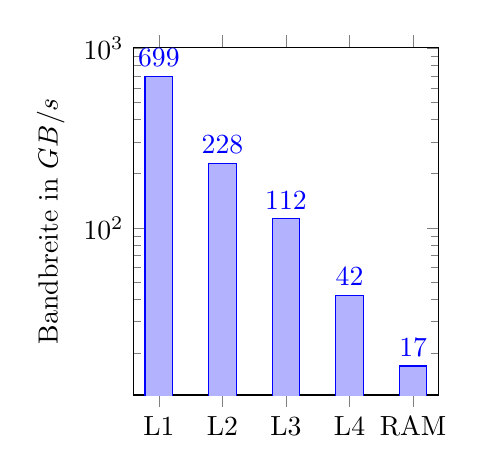
\begin{tikzpicture}
	\begin{axis}[
			height=6cm,
			width=0.45\textwidth,
			ybar,
			ymode=log,
			%extra tick style={grid=major},
			ylabel={Bandbreite in $GB/s$},
			symbolic x coords={L1, L2, L3, L4, RAM},
			xtick=data,
			nodes near coords,
			nodes near coords align={vertical}
		]
		\addplot+[point meta=explicit symbolic] 
		coordinates {
			(L1, 699) [699]
			(L2, 228) [228]
			(L3, 112) [112]
			(L4, 42) [42]
			(RAM, 17) [17]
		};
	\end{axis}
\end{tikzpicture}

		\label{fig:bas:memperf}
	}
	\hfill
	\subfigure[Cachegröße]{
		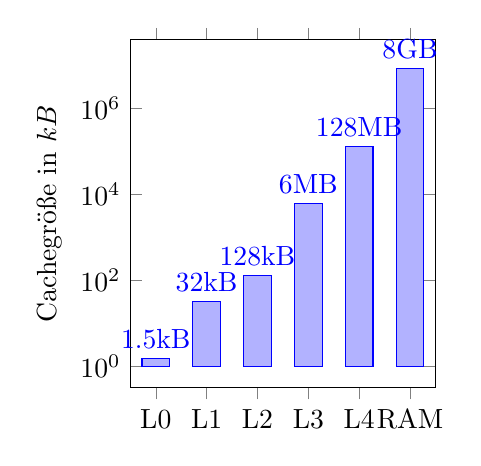
\begin{tikzpicture}
	\begin{axis}[
			height=6cm,
			width=0.45\textwidth,
			ybar,
			ymode=log,
			%log ticks with fixed point,
			%extra tick style={grid=major},
			ylabel={Cachegröße in $kB$},
			symbolic x coords={L0, L1, L2, L3, L4, RAM},
			xtick=data,
			nodes near coords,
			nodes near coords align={vertical}
		]
		\addplot+[point meta=explicit symbolic] coordinates 
		{
			(L0, 1.5) [1.5kB]
			(L1, 32) [32kB] 
			(L2, 128) [128kB]
			(L3, 6144) [6MB]
			(L4, 131072) [128MB]
			(RAM, 8388608)[8GB]
		};
	\end{axis}
\end{tikzpicture}

		\label{fig:bas:memsize}
	}
	\hfill
	\caption{Beispiel: Spitze der Cachehierarchie in einem aktuellen Rechner mit dem ``Intel Mobile Haswell (CrystalWell)'' Prozessor und 2x4GB DDR3 1600MHz Arbeitsspeicher\cite{cache}.}
	\label{fig:bas:sizeperf}
\end{figure}


% Funktionsweise
Der Leistungsgewinn entsteht nur, wenn die benötigten Daten im Cache liegen.
Bei einem Lesezugriff prüft das System, ob die benötigten Daten im Cache liegen. 
Wenn das der Fall ist, nennt man das ein Cache-Hit, werden sie aus dem Cache gelesen, andernfalls, beim Cache-Miss, werden sie erst vom Speichermedium in den Cache eingelesen und dann aus dem Cache gelesen. 

Der Einsatz von Caches kann zu einer scheinbaren Überschreitung des theoretischen maximalen Leistung der Komponenten führen, wenn die benötigten Daten bereits im Cache liegen. 
In diesem Fall ist der E/A-Zugriff auf den Massenspeichermedium überflüssig und wird übersprungen. 

Das Cache-Systems verfolgt das Ziel die bald benötigten Daten im Cache bereit zu halten.
Dazu nutzt es vor allem die zeitliche und räumliche Lokalitäten.
% erneuter Zugriff
Bei zeitlicher Lokalität wird ein Speicherbereich in den Cache geladen und bleibt dort, wenn das Cache-System davon ausgeht, dass es bald wieder benutzt wird.
% Zugriff auf die nachfolgenden Adressen
Bei räumlicher Lokalität werden in den Cache auch die benachbarten Speicherbereiche geladen, wenn das Cache-System davon ausgeht, dass sie bald benötigt werden. 
Z.B. wenn aus dem Code hervorgeht, dass ein Array sequentiell in einer Schleife verarbeitet wird.

Neben den tradidionellen Cachehierarchie gibt es noch weitere Formen, die nach dem selben Prizip funktionieren, sich aber nicht so einfach in die Cachehierarchie eingliedern lassen, z.B. SSD-Cachesysteme, Auslagerungsdatei, HTTP-Caching. Vom Prizip her funktionieren sie ähnlich, wie hier beschriebene Caches.



%\subsection{Leistungsanalyse}
%Für Leistungsanalyse benötigt man spezielle Werkzeuge, die das Programmverhalten protokollieren und analysieren. Die Ursache für die Leistungseinbußen sollen nach Möglichkeit herauskristallisiert werden.

%Die Optimierung kann darauf ausgerichtet werden, möglichst aus einer höheren Cachehierarchie die Daten zu bekommen. 

% anomaly detection
%\todo{Anomaly detection}
%EVTL!!! Wahrscheinlich langt es in der Einleitung
%Wie passiert das Vampir etc.

% Betriebssystem und Anwendungen




\subsection{SIOX-Aktivitäten}
Die SIOX-Aktivitäten sind Datenstrukturen, die Informationen über die E/A-Operationen beinhalten.
Die aktuelle Version arbeitet bereits mit HDF5-, NETCDF4-, MPI- und POSIX-Schnittstellen.
Die Aktivitäten dienen als eine Basis für die Leistungsanalyse und werden in diesem Abschitt detailiert betrachtet.

Die \tabref{tab:bas:activity} listet grob alle Bestandteile einer SIOX-Aktivität.
Der Typ und der Name wurden direkt aus dem Quellcode übernommen und kurz beschrieben.
Da in dieser Arbeit nur die POSIX-Schnittstelle betrachtet wird, werden nicht alle Bestandteile benötigt.
Die nicht verwendeten Bestandteile wurde in der Tabelle ausgegraut.

\begin{table}[h]
	\centering
	\begin{scriptsize}
		\begin{tabular}{l | l | l}
			Typ & Name & Beschreibung \\
			\hline
			\lstinline{ActivityID}                                              & \lstinline{aid}                                                & Eindeutiger Bezeichner \\
			\lstinline{UniqueComponentActivityID}                               & \lstinline{ucaid}                                              & Typ der E/A-Operation \\
			\lstinline{Timestamp}                                               & \lstinline{time_start}                                         & Startzeit in Nanosekunden\\
			\lstinline{Timestamp}                                               & \lstinline{time_stop}                                          & Stopzeit in Nanosekunden \\
			\lstinline{vector<ActivityID>}                                      & \lstinline{parentArray}                                        & Ausgangs-E/A-Operationen \\
			\lstinline[basicstyle=\ttfamily\color{gray}]{vector<RemoteCall>}    & \lstinline[basicstyle=\ttfamily\color{gray}]{remoteCallsArray} & \textcolor{gray}{\textit{-}} \\
			\lstinline{vector<Attribute>}                                       & \lstinline{attributeArray}                                     & Parameter, Rückgabewert, usw. \\
			\lstinline[basicstyle=\ttfamily\color{gray}]{RemoteCallIdentifier*} & \lstinline[basicstyle=\ttfamily\color{gray}]{remoteInvoker}    & \textcolor{gray}{\textit{-}} \\
			\lstinline[basicstyle=\ttfamily\color{gray}]{ActivityError}         & \lstinline[basicstyle=\ttfamily\color{gray}]{errorValue}       & \textcolor{gray}{\textit{-}}
		\end{tabular}
	\end{scriptsize}
	\caption{Zusammensetzung der SIOX-Aktivitäten. (Die ausgegrauten Bestandteile sind nicht relevant für diese Arbeit.)}
	\label{tab:bas:activity}
\end{table}

Ganz besonders interessant sind die drei POSIX-Operationstypen: Eingabe-, Ausgabe- und Positionierungsoperationen, denn in den meisten Fällen bestimmen sie die E/A-Leistung.
%https://en.wikipedia.org/wiki/C_file_input/output
Um einmal zu zeigen wie diese Operationen in den SIOX-Aktivitäten behandelt werden schauen wir uns jeweils einen Vertreter von jedem Typ an, nämlich \lstinline{fread}-, \lstinline{fwrite}- und \lstinline{fseek}-Operation (\lstref{lst:des:posixops}).

\begin{lstlisting}[language=C, belowcaptionskip=1\baselineskip, caption={POSIX-Operationen}\label{lst:des:posixops}]
size_t fread(void *ptr, size_t size, size_t nmemb, FILE *stream);
size_t fwrite(const void *ptr, size_t size, size_t nmemb, FILE *stream);
int fseek(FILE *stream, long offset, int whence);
\end{lstlisting}

Die \lstinline{aid}, \lstinline{time_start} und \lstinline{time_stop} Elemente sind von Funktion her trivial. 
ucaid ist als eine Zahl kodierter Operationstyp und ist ebenfalls trivial. 
Spannend wird es bei \lstinline{parentArray} und \lstinline{attributeArray}.

Das Attribute \lstinline{parentArray} verweist auf die Ausgangs-Aktivitäten, d. h. auf die Aktivitäten mit der der Zugriff auf eine bestimmte Datei begonnen hat.
Bei POSIX handelt es sich typischerweise um die open-Aktivität.
Die Aktivitäten mit dem gleichen parentArray bilden eine Gruppe und, wenn zeitlich angeordnet, eine Aktivitätensequenz auf eine bestimmte Datei.
Wenn eine Datei mehrmals geöffnet wurde und die Zugriffe über verschiedene FileHandler erfolgen, dann sind auch die parentArray's unterschiedlich.
Hat eine Aktivität keine Ausgangsaktivität, wie z. B. open-Aktivität, dann ist parentArray leer.


Das Attribute attributeArray beinhaltet Informationen über den Systemaufruf.
Das können die Funktionsparameter, der Rückgabewert, diverse Laufzeitinformationen usw. sein.
Der Inhalt von attributeArray ist spezifisch für die E/A-Operation. 

\begin{table}[h]
	\centering
	\begin{tabular}{l | l}
		Attribute & Wert\\
		\hline
		POSIX/quantity/BytesToWrite & 4\\
		POSIX/descriptor/FilePointer & 28317504\\
		POSIX/data/MemoryAddress & 4233230\\
		POSIX/quantity/BytesWritten & 4
	\end{tabular}
	\caption{Attribute und Beispielwerte einer write-Operation.}
\end{table}

\begin{table}[h]
	\centering
	\begin{tabular}{l | l}
		Attribute & Wert\\
		\hline
		POSIX/quantity/BytesToRead & 100\\
		POSIX/data/MemoryAddress & 22192128\\
		POSIX/descriptor/filehandle & 0\\
		POSIX/quantity/BytesRead & 100\\
	\end{tabular}
	\caption{Attribute und Beispielwerte einer read-Operation.}
\end{table}

\begin{table}[h]
	\centering
	\begin{tabular}{l | l}
		Attribute & Wert\\
		\hline
		POSIX/descriptor/filehandle & 4\\
		POSIX/file/position & 0\\
	\end{tabular}
	\caption{Attribute und Beispielwerte einer read-Operation.}
\end{table}



\subsubsection{Erzeugung von Aktivitätensequenzen}

Die Offline-Analyse wird in drei Schritten durchgeführt.

Im ersten Schritt werden die Aktivitäten einer Anwendung aufgezeichnet und in einer Spurdatei gespeichert \figref{fig:bas:get_trace}. 
Dazu wir das Siox-Instrumentierungstool verwendet.
\begin{figure}[h]
	\centering
	\begin{tikzpicture}
	[
		remember picture,
		>=latex reversed,
		organism/.style={draw,rounded corners},
		node distance=5mm and 5mm
	]
	
	\node
		[organism]
		(app)
		{Anwendung};
	\node
		[organism,right=of app]
		(inst)
		{Instrumentierung};
	\node
		[organism,right=of inst]
		(tracefile)
		{Spurdatei};

	\path
		[->, >=latex]
		(app)	edge	(inst)
		(inst)	edge	(tracefile);


\end{tikzpicture}

	\caption{Erstellung einer Spurdatei.}
	\label{fig:bas:get_trace}
\end{figure}

Im zweiten Schritt werden die Aktivitäten ausgewertet. 
Dazu wird die erstellt Spurdatei mit siox-trace-reader eingelesen, der dann die Aktivitäten an den Analyse-Plugin weiterleitet.
Das Plugin startet dann den Lernprozess.
Die Ergenisse im diesen Schritt sind zwei Entscheidungsbäume: das eine für die Leistungsvorhersage und das andere für die Klassifizierung.

\begin{figure}[h]
	\centering
	\begin{tikzpicture}
	[
		remember picture,
		>=latex reversed,
		organism/.style={draw,rounded corners},
		node distance=5mm and 5mm
	]
	
	\node
		[organism]
		(file)
		{Spurdatei};
	\node
		[organism,right=of file]
		(tracereader)
		{SIOX};
	\node
		[organism,right=of tracereader]
		(ke)
		{Analyse-Plugin};
	\node
		[organism,right=of ke]
		(result)
		{Ergebnisse};

	\path
		[->, >=latex]
		(file)	edge	(tracereader)
		(tracereader)	edge	(ke)
		(ke) edge (result);


\end{tikzpicture}

	\caption{Vorhersage}
	\label{fig:bas:results}
\end{figure}

Im dritten Schritt wird wieder eine Spurdatei (die gleiche oder eine andere) eingelesen und vom Plugin ausgewertet.
Die Ergebnisse sind Vorhersagen der Leistungswerte, Klassenzuordnung und Anomalien.

Die Anomalien liefern Hinweise auf besondere Stellen.
Diese Stellen werden untersucht und nach Möglichkeit Rückschlüsse gezogen.

\bigskip

%\todo{Kurze Zusammenfassung und Überleitung, ein paar Zeilen}
\textit{In diesem Kapitel haben wurden die Arbeit relevanten Begriffe, Techniken und Technologien behandelt. 
In den folgenden drei Kapiteln werden kombiniert, um Daten zu erzeugen und auszuwerten.}

